
%\graphicspath{{img}}
\begin{tcolorbox}
Die Produktfunktionen beschreiben jede einzelne Funktion des Produkts mittels Anwendungsfalldiagrammen und Anwendungsfalltabellen.
Diese sollen möglichst ausschlaggebend für das zu entwickelnde System sein und nicht simple Produktfunktionen wie z.B. Login, Account erstellen, Gruppe beitreten, Passwort ändern oder ähnliches zeigen.
\autoref{fig:anwendungsfall-app-tabelle-xx-1} stellt eine exemplarische Tabelle für die Beschreibung eines Anwendungsfalls dar. Stil und Formatierung sind variabel. Nicht jede Zelle muss immer gefüllt sein.
\\\\
In  Tabelle~\autoref{fig:akteur-tabelle} werden alle auftretenden Akteure beschrieben.


\end{tcolorbox}

\begin{figure}[h]
	\centering
	
	\begin{tabularx}{\textwidth}{ p{.2\textwidth} | p{.2\textwidth} | X }
		\textbf{Akteur} & \textbf{Beschreibung} & \textbf{Verwendet in Anwendungsfall} \\ \hline
		Informatiker & Programmiert tolle Sachen & Programmieren, Kaffee trinken, Schlafen
	\end{tabularx}
	
	\caption{Beschreibung der Akteure}
	\label{fig:akteur-tabelle}
\end{figure}


%%%%%%%%%%%%%%%
%% Anwendungsfall 1 %%
%%%%%%%%%%%%%%%

\section{Anwendungsfalldiagramm - App}

\begin{figure}[h]
	\centering
    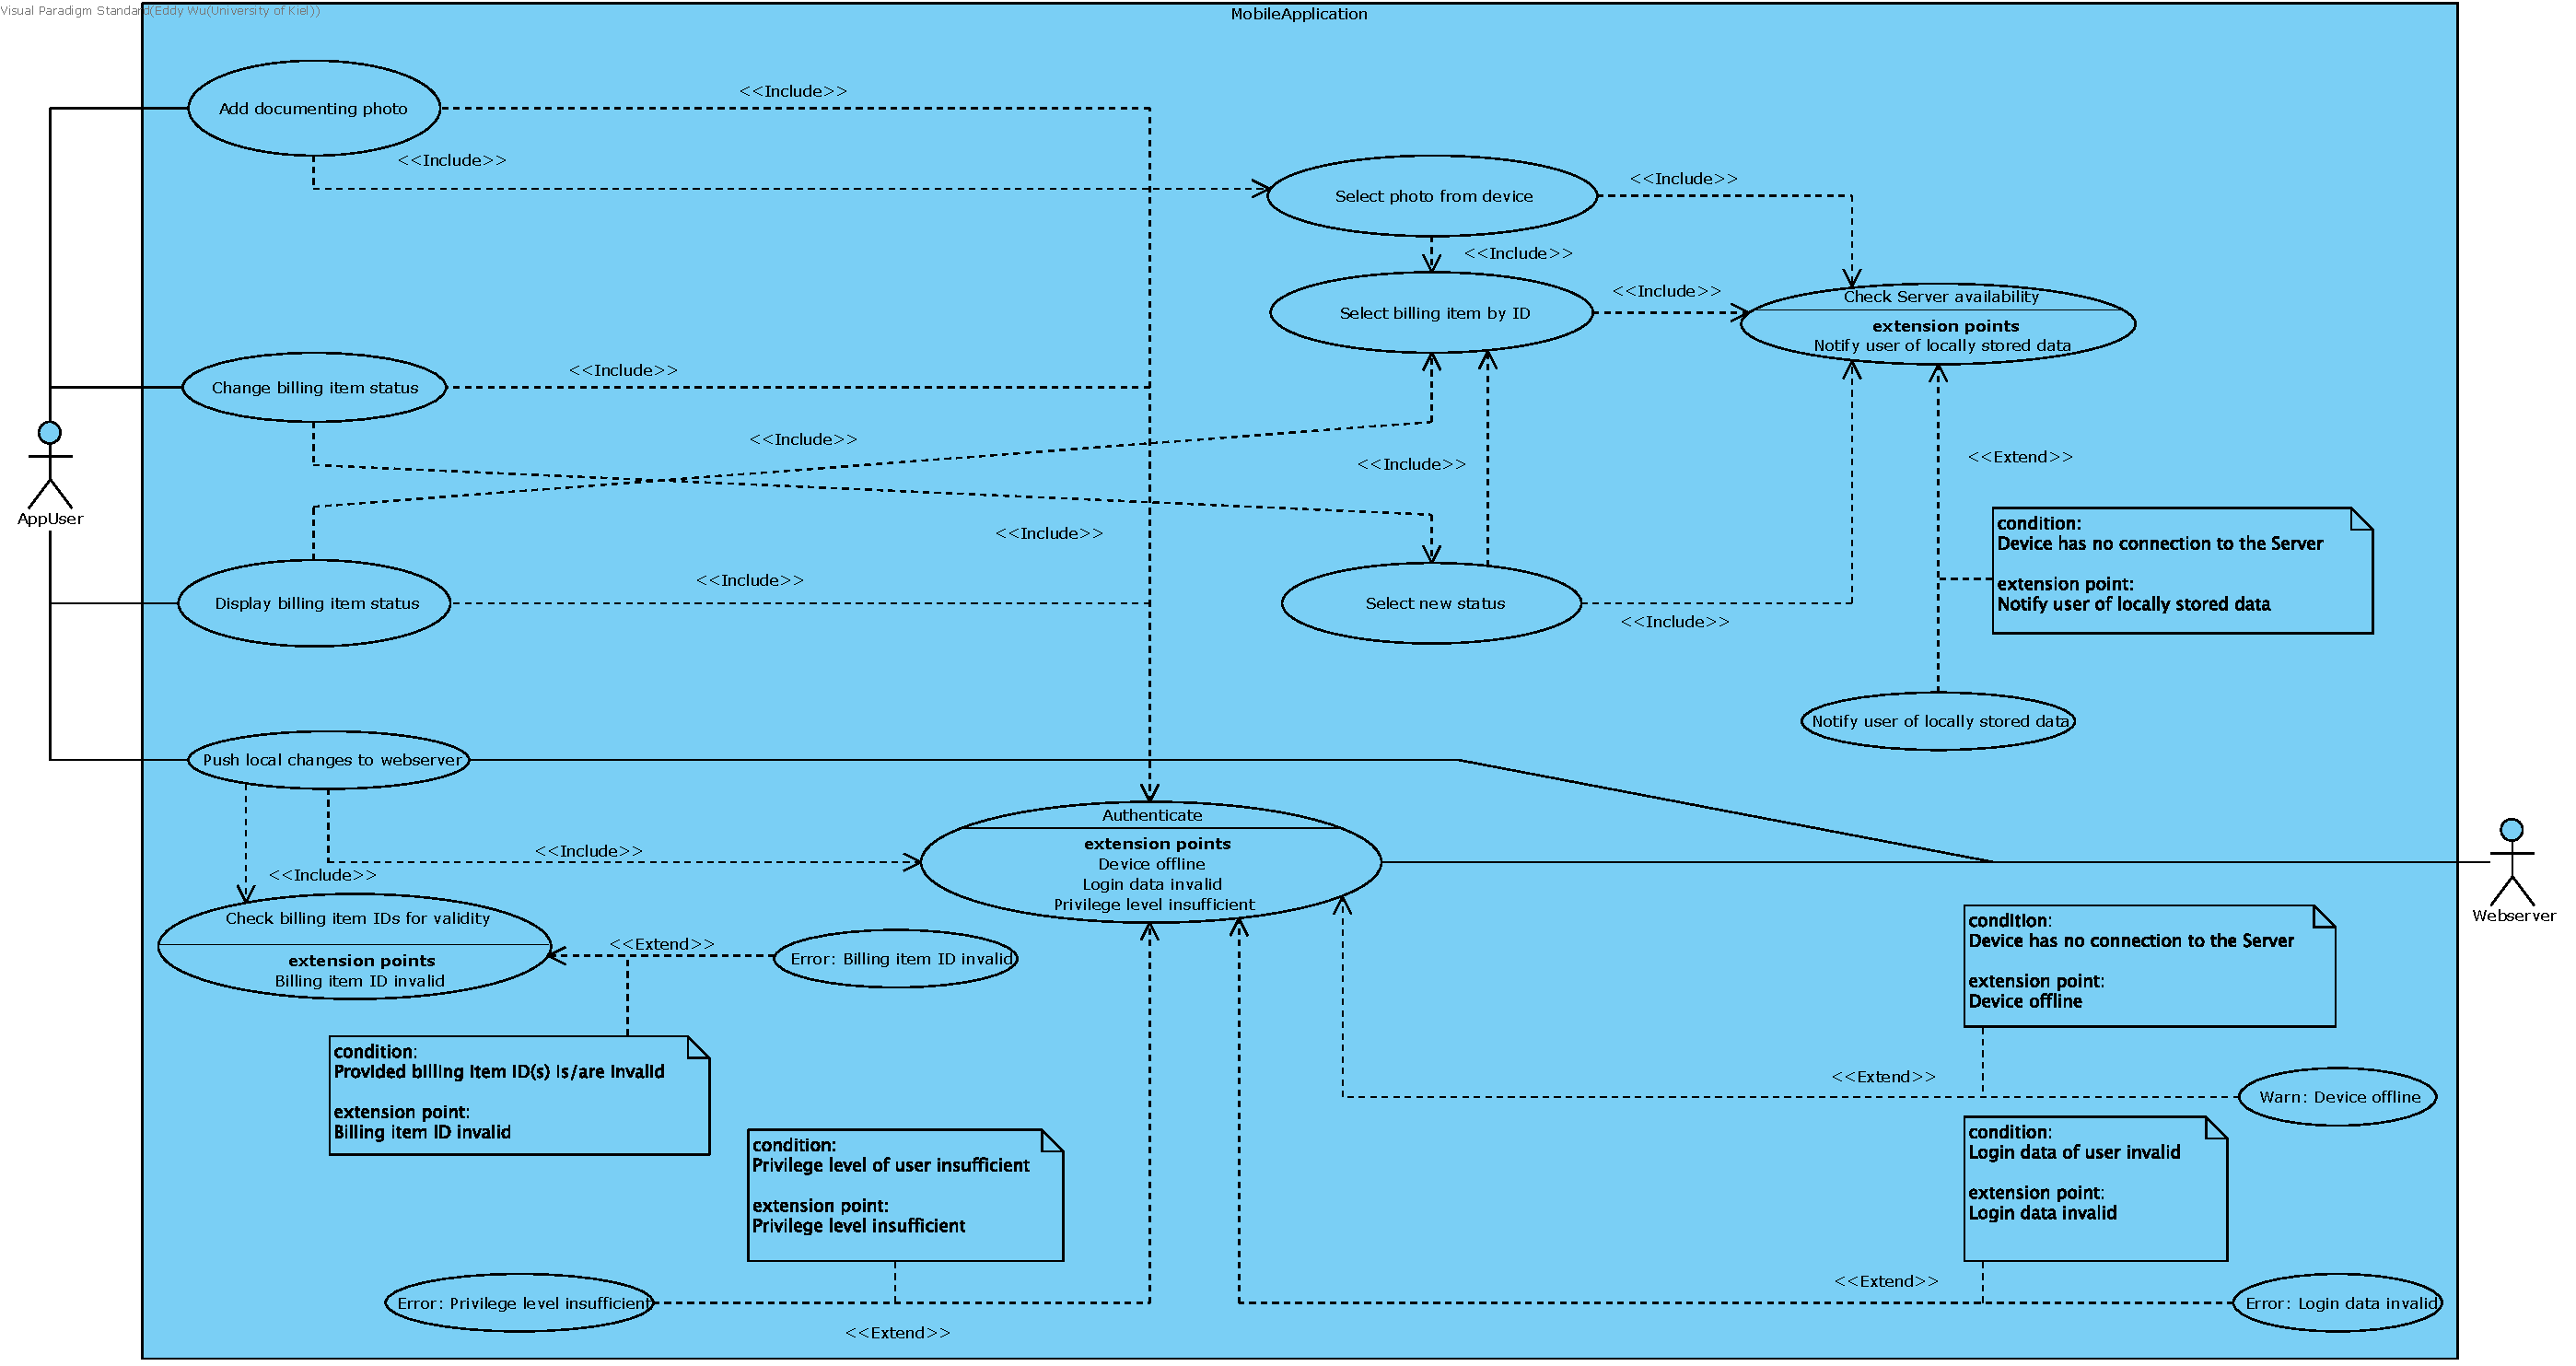
\includegraphics[width=\linewidth]{diagrams/Mobile_Application.pdf}
	\caption{Anwendungsfalldiagramm - App}
	\label{fig:anwendungsfalldiagramm-app}
\end{figure}

\newpage

\begin{figure}[h]
	\centering
	\begin{tabularx}{\textwidth}{ X | X }
		\textbf{Anwendungsfall ID} & XX-1 \\ \hline
		\textbf{Anwendungsfallname} & Hier steht ein Name. \\ \hline
		\textbf{Initiierender Akteur} & Informatiker \\ \hline
		\textbf{Weitere Akteure} & Designer, Techniker  \\ \hline
		\textbf{Kurzbeschreibung} & Hier steht eine Kurzbeschreibung.  \\ \hline
		\textbf{Vorbedingungen} & -  \\ \hline
		\textbf{Nachbedingungen} & Y trifft zu.  \\ \hline
		\textbf{Ablauf} &
			\begin{enumerate}
				\item Erster ganzer Satz.
				\item Zweiter ganzer Satz.
			\end{enumerate} \\ \hline
		\textbf{Alternative} &
				\begin{enumerate}
					\item Erster ganzer Satz.
					\item Zweiter ganzer Satz.
				\end{enumerate}  \\ \hline
		\textbf{Ausnahme} &
				\begin{enumerate}
					\item Erster ganzer Satz.
					\item Zweiter ganzer Satz.
				\end{enumerate}  \\ \hline
		\textbf{Benutzte Anwendungsfälle} & YY-1 (oder Name) \\ \hline
		\textbf{Spezielle Anforderungen} & - \\ \hline
		\textbf{Annahmen} & -
	\end{tabularx}
	\caption{Anwendungsfall XX-1}
	\label{fig:anwendungsfall-app-tabelle-xx-1}
\end{figure}

\newpage


%%%%%%%%%%%%%%%
%% Anwendungsfall 2 %%
%%%%%%%%%%%%%%%

\section{Anwendungsfalldiagramme - Web}

\begin{figure}[h]
	\centering
	\includesvg[inkscapelatex=false, width=\linewidth]{diagrams/Acc_Management_Web}	
	\caption{Anwendungsfalldiagramm - Account Management Webserver}
	\label{fig:anwendungsfalldiagramm-server}
\end{figure}

\newpage

\begin{figure}[h]
	\centering
	\begin{tabularx}{\textwidth}{ X | X }
		\textbf{Anwendungsfall ID} & XX-1 \\ \hline
		\textbf{Anwendungsfallname} & Hier steht ein Name. \\ \hline
		\textbf{Initiierender Akteur} & Informatiker \\ \hline
		\textbf{Weitere Akteure} & Designer, Techniker  \\ \hline
		\textbf{Kurzbeschreibung} & Hier steht eine Kurzbeschreibung.  \\ \hline
		\textbf{Vorbedingungen} & -  \\ \hline
		\textbf{Nachbedingungen} & Y trifft zu.  \\ \hline
		\textbf{Ablauf} &
		\begin{enumerate}
			\item Erster ganzer Satz.
			\item Zweiter ganzer Satz.
		\end{enumerate} \\ \hline
		\textbf{Alternative} &
		\begin{enumerate}
			\item Erster ganzer Satz.
			\item Zweiter ganzer Satz.
		\end{enumerate}  \\ \hline
		\textbf{Ausnahme} &
		\begin{enumerate}
			\item Erster ganzer Satz.
			\item Zweiter ganzer Satz.
		\end{enumerate}  \\ \hline
		\textbf{Benutzte Anwendungsfälle} & YY-1 (oder Name) \\ \hline
		\textbf{Spezielle Anforderungen} & - \\ \hline
		\textbf{Annahmen} & -
	\end{tabularx}
	\caption{Anwendungsfall XX-1}
	\label{fig:anwendungsfall-server-tabelle-xx-1}
\end{figure}

%%%%%%%%%%%%%%%
%% Anwendungsfall 3 %%
%%%%%%%%%%%%%%%

%\section{Anwendungsfalldiagramme - Diagrammverwaltung (Web)}

\begin{figure}[h]
	\centering
	\includesvg[inkscapelatex=false, width=\linewidth]{diagrams/Acc_Management_Web}	
	\caption{Anwendungsfalldiagramm - Diagrammverwaltung}
	\label{fig:anwendungsfalldiagramm-diagrammverwaltung}
\end{figure}

\newpage

\begin{figure}[h]
	\centering
	\begin{tabularx}{\textwidth}{ X | X }
		\textbf{Anwendungsfall ID} & XX-1 \\ \hline
		\textbf{Anwendungsfallname} & Diagrammverwaltung von Diagrammen. \\ \hline
		\textbf{Initiierender Akteur} & Systemadministrator \\ \hline
		\textbf{Weitere Akteure} & Organisationsadministrator, Mitarbeiter \\ \hline
		\textbf{Kurzbeschreibung} & Darstellung und mögliche Filterung der vom Server automatisch erzeugten Diagramme innerhalb der Webapplikation.  \\ \hline
		\textbf{Vorbedingungen} & Funktionierende Internetverbindung, bestätigte Berechtigungen (Authentifiziert)  \\ \hline
		\textbf{Nachbedingungen} &  -  \\ \hline
		\textbf{Ablauf} &
		\begin{enumerate}
			\item Authentifizieren.
			\item Darstellen eines allgemeinen (alle Leistungspunkte umfassend) Diagrammes zu einem oder mehreren Verträgen.
		\end{enumerate} \\ \hline
		\textbf{Alternative} &
		\begin{enumerate}
			\item Authentifizieren.
			\item Filtern nach bestimmten Kriterien.
			\item Darstellen eines Diagrammes zu einem oder mehreren Verträgen.
		\end{enumerate} % \hline
		\begin{enumerate}
			\item Authentifizieren.
			\item Diagramm zum Baufortschritt eines Projektes anzeigen.
		\end{enumerate}  \\ \hline
		\textbf{Ausnahme} &
		\begin{enumerate}
			\item Keine erfolgreiche Authentifizierung.
			\item Keine ausreichenden Berechtigungen.
			\item Vertrag/Projekt nicht vorhanden.
		\end{enumerate}  \\ \hline
		\textbf{Benutzte Anwendungsfälle} & Benutzerverwaltung (YY-1) \\ \hline
		\textbf{Spezielle Anforderungen} & Besitz einer Rolle mit entsprechenden Berechtigungen. \\ \hline
		\textbf{Annahmen} & -
	\end{tabularx}
	\caption{Anwendungsfall XX-1}
	\label{fig:anwendungsfall-diagrammverwaltung-tabelle-xx-1}
\end{figure}